\section{Background}\label{sec:background} 
\begin{figure}[t]
  \centering
  \vspace{2mm}
  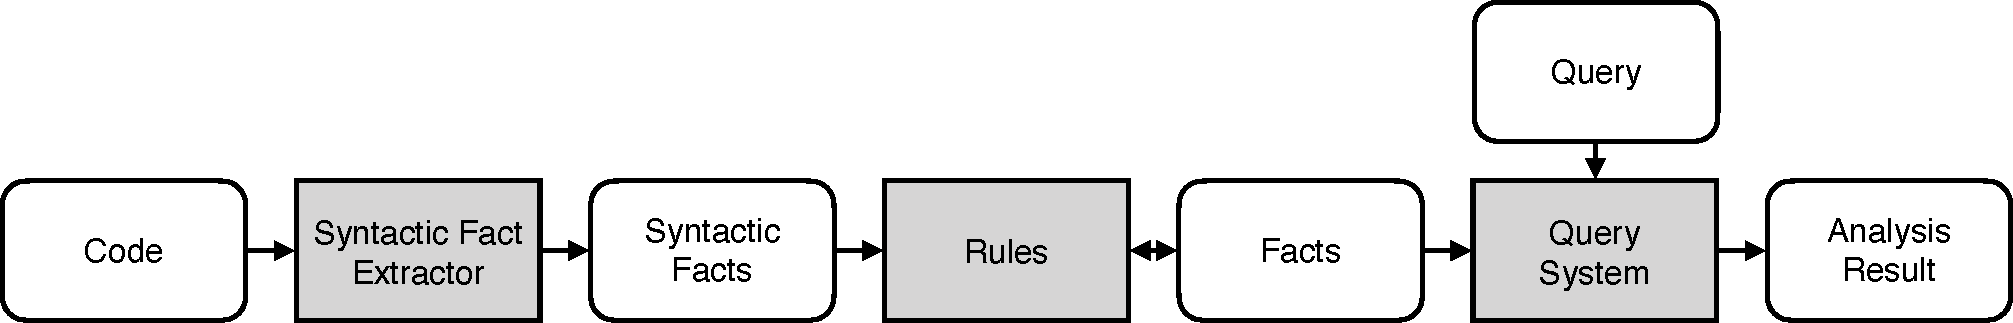
\includegraphics[width=0.94\textwidth]{img/ov1.pdf}
%  \vspace*{-1.5em}
  \caption{Overview of a declarative static analysis}
  \label{fig:ov1}
%\vspace*{-.5em}
\end{figure}

Figure~\ref{fig:ov1} presents the overview of how a declarative static
analysis works.  The analysis consists of three steps.  First, a given program
gets converted into syntactic facts. 
Second, new facts are generated by iteratively applying rules to the set of
known facts, until no new facts are derived.  
Finally, the query system takes a query and evaluates the rules with the given
facts, producing an analysis result for the query. 
The following paragraphs explain each step in detail, with examples written in
the Datalog-like syntax.

%Figure~\ref{fig:ov1} presents the overview of how a declarative style analysis
%works. The analysis consists of three steps.  First, a given program gets
%converted into database of syntactic facts.  Second, the rules that generate
%new facts are defined, and a declarative language engine evaluates the rules
%with the given facts, producing new facts.  Finally, the query is executed to
%extract all the facts that meet certain conditions, which correspond to the
%analysis result.

\textbf{Step 1: Extracting syntactic facts.}
The first step is to extract syntactic facts from a given program source.
Syntactic facts include facts about certain AST nodes and
parent-child relationships between nodes. 
For example, consider the following code:

\begin{lstlisting}[style=mcpp]
int f() {
  return 42;
}

int val = f();
\end{lstlisting}

For function definitions, the Syntactic Fact Extractor can extract syntactic
facts of a form \rcode{ Return(functionName, value)}, where \rcode{Return}
denotes the relation between two nodes, \rcode{functionName} denotes the name of a
function, and \rcode{value} denotes the return value of the function.
Therefore, the extractor can extract the fact \rcode{ Return("f", 42)} from
the code.  
Another example syntactic fact is \rcode{ Call(callExpr, functionName)}, which
denotes that a node \rcode{ callExpr} is a call expression to a function named
\rcode{ functionName}.
For instatnce, the extractor can extract the following syntactic fact from the
code: \rcode{ Call(f(), "f")}.

%\inred{
%These syntactic facts serve as building blocks for the
%common Intermediate Representation (IR) of multiple languages.
%Compared to other IRs, this declarative-style IR has a few advantages.
%First, extracting information from source code in this format does not
%require any understanding of the language semantics, which imposes
%almost no performance overhead beyond parsing the source code.
%Second, the syntactic facts can be utilized easily in other kinds of
%analysis, since they are simple information that can be freely
%manipulated when defining new rules. Therefore, even when we use a different
%client analysis, we can reuse the extracted syntactic facts
%without re-extracting them from the source code.}

\smallskip
\textbf{Step 2: Deriving new facts by applying rules.}
The next step is to derive new facts from known facts by applying rules.
A rule defines a relation of that a fact, called {\it derived fact}, can be
derived from a set of facts, called {\it base fact}. 
If all the base facts belong to known facts, the derived fact is generated and
added to the known facts by the rule.
This process of deriving new facts is repeated, until no more new facts are
found.
%A rule indicates that if a certain facts are known, then a new rule can be
%generated and added to the set of known facts. This process of generating
%new facts is repeated, until no more new facts are found.


For example, consider a fact \rcode{ Step(x, y)} that denotes a direct dataflow
from a node \rcode{ x} to a node \rcode{ y}. 
Here, nodes represent program entities that evaluates in to runtime values,
such as variables, literals, and function parameters. 
A direct dataflow can be established via the relation between a function call
expression and its callee's return, as represented by the following rule.
\begin{lstlisting}[style=mrule]
Step(ret, callExpr) :- Call(callExpr, functionName), Return(functionName, ret)
\end{lstlisting}

\noindent
This rule indicates that when we have two syntactic facts, \rcode{ Calls(callExpr, functionName)},
and \rcode{ Returns(functinName, retVar) }, then the new fact \rcode{ Step(retVar, call) } can be derived.
Since we already have \rcode{ Calls(f(), "f")} and \rcode{ Returns("f", 42) } as the base facts,
we can derive the new fact, \rcode{ Step(42, f()) }.

The newly derived facts \rcode{ Step} can also be used to derive new facts.
For example, we can think of another \rcode{ Flow(x, z)} that denotes a dataflow from a
node \rcode{ x} to a node \rcode{ z}.
We can define rules for generating the fact as the transitive closure of \rcode{ Step}:

\begin{lstlisting}[style=mrule]
Flow(x, z) :- Step(x, z)
Flow(x, z) :- Step(x, y), Flow(y, z)
\end{lstlisting}

\noindent
The first rule indicates that the fact \rcode{ Flow(x, z)} is derived if the
fact \rcode{ Step(x, z)} belongs to known facts, and the second rule indicates
that the fact \rcode{ Flow(x, z)} is also derived if the two facts \rcode{
Step(x, y)} and \rcode{ Flow(y, z)} belong to known facts.
When a new fact is derived by rules, the fact is added to the known facts and
used as a base fact iteratively to derive other new facts.
%\inred{ \sout {
%The rules are usually
%evaluated in a bottom-up and modular manner, that is, each rule is evaluated
%one by one, after every rule it depends on is evaluated.
%}}

%The next step is to define rules to generate new facts out of known facts.
%%This step corresponds to actually implementing the algorithm of a
%%static analysis in a declarative style.
%For example, recall that we can define a call graph
%\rcode{ CallEdge(l1, l2)} using the facts
%named \rcode{ FunctionAt} and \rcode{ CallAt}.
%The defined rules are evaluated with declarative engines to finding all possible
%facts that can be derived. The rules are usually evaluated in a bottom-up
%and modular manner. Each rule is evaluated one-by-one, after every
%rule it depends on is evaluated. 

\smallskip
\textbf{Step 3: Performing queries.}
The final step is to perform the query via the query system.  
A query is a set of facts containing variables, and the query system finds
every variable assignment that makes the facts in the query belong to known
facts.
This step corresponds to actually obtaining the final result of a static
analysis in a declarative style.  
For example, one can make a specific query:

\begin{lstlisting}[style=mrule]
?- Flow(42, X)
\end{lstlisting}

\noindent
that queries all nodes into which the integer literal {\tt 42} flows.
When accepting the query as an input, the query system finds every value
\rcode{ v} such that \rcode{ Flow(42, v)} belongs to known facts generated in
the previous step. 
In this example, the query would give the query result
\rcode{ X\ $\in$ \{f(), val\}}.

%The final step is to perform queries via query system.
%The result of the query corresponds to actual result of client analysis.
%A query consists of set of facts, where some of the facts would have
%varaibles as arguments. Given a query, the query sytem will find all possible
%assignment on variables, that will make every facts would hold under
%the assignment.
%\newpage
